% FADO --- CISUC template, Beamer version.
% Compiles with pdfLaTeX, XeLaTeX, or LuaLaTeX (run twice for the TikZ overlays).
\documentclass[aspectratio=169]{beamer}
\usepackage{geometry}
\geometry{paperwidth=13.333in,paperheight=7.5in}
\usepackage{iftex}
\usepackage{tikz}
\usetikzlibrary{arrows.meta}
\usepackage{booktabs}
\usepackage{multirow}
\usepackage{amsmath}
\usepackage{array}
\usepackage{amsmath, amsthm}

% ---- fonts (engine-agnostic; TeXLive-bundled Helvetica/Courier clones, no fontspec) ----
\ifPDFTeX\usepackage[utf8]{inputenc}\fi
\usepackage[T1]{fontenc}
\usepackage{textcomp}
\usepackage{tgheros}   % Helvetica clone (Arial-like) sans
\usepackage{tgcursor}  % Courier clone mono
\renewcommand{\familydefault}{\sfdefault}
\newcommand{\monofont}{\ttfamily}

% ---- colours ----
\definecolor{cred}{HTML}{DA0725}
\definecolor{ink}{HTML}{141414}
\definecolor{body}{HTML}{262626}
\definecolor{grey}{HTML}{9A9A9A}
\definecolor{lgrey}{HTML}{C4C4C4}
\definecolor{rulec}{HTML}{2A2A2A}
\definecolor{green}{HTML}{2E9E5B}
\definecolor{amber}{HTML}{C77A18}

\setbeamercolor{normal text}{fg=body}
\setbeamercolor{itemize item}{fg=cred}
\setbeamercolor{itemize subitem}{fg=cred}
\setbeamercolor{itemize subsubitem}{fg=cred}
\setbeamercolor{enumerate item}{fg=cred}
\setbeamercolor{enumerate subitem}{fg=cred}
\setbeamercolor{enumerate subsubitem}{fg=cred}
\setbeamercolor{item projected}{fg=cred}
\setbeamertemplate{navigation symbols}{}
\setbeamersize{text margin left=0.85in,text margin right=0.85in}

% ---- running header (shown on non-plain frames) ----
\newcommand{\hdrsec}{}
\newcommand{\hdrpg}{}
\newcommand{\pageset}[2]{\renewcommand{\hdrsec}{#1}\renewcommand{\hdrpg}{#2}}
\setbeamertemplate{headline}{%
  \vskip3mm%
  \makebox[\paperwidth][c]{%
    \hspace{9mm}%
    \parbox[t]{4.2in}{\monofont\color{grey}\fontsize{9}{11}\selectfont
      FADO: A Reaction Controller for Fairness-\\ Aware Online Learning Under Concept Drift}%
    \hfill
    \parbox[t]{4.2in}{\centering\monofont\color{grey}\fontsize{10}{12}\selectfont \hdrsec}%
    \hfill
    \parbox[t]{2.6in}{\raggedleft\monofont\fontsize{13}{15}\selectfont
      \textbf{\color{ink}\hdrpg}{\color{grey}/12}}%
    \hspace{9mm}%
  }%
}
\setbeamertemplate{theorems}[numbered]
\makeatletter
\setbeamertemplate{theorem begin}{%
  \begin{\inserttheoremblockenv}
    {%
      \centering
      \inserttheoremname
      \inserttheoremnumber
      \ifx\inserttheoremaddition\@empty\else\ (\inserttheoremaddition)\fi%
    }%
}
\makeatother
\setbeamertemplate{proof begin}{\begin{block}{\insertproofname}\sffamily}
\setbeamertemplate{footline}{}
\setbeamertemplate{frametitle}{}

% ---- helpers (absolute placement via TikZ overlay) ----
% \tb{width-in}{x-in}{y-in}{content}  --- anchored top-left at (x,y) from page NW
% optional #1 = extra node options (use font=... for large text so spacing scales)
\newcommand{\tb}[5][]{\begin{tikzpicture}[remember picture,overlay]%
  \node[anchor=north west,inner sep=0pt,outer sep=0pt,text width=#2in,align=left,#1]
    at ([xshift=#3in,yshift=-#4in]current page.north west){\raggedright #5\par};\end{tikzpicture}}
\newcommand{\fs}[2]{\fontsize{#1}{#2}\selectfont}
\newcommand{\hrl}[3]{\tb{#3}{#1}{#2}{{\color{lgrey}\rule{#3in}{0.9pt}}}}
% square outline cell with centred label: \boxcell{x}{y}{size-in}{label}
\newcommand{\boxcell}[4]{\begin{tikzpicture}[remember picture,overlay]%
  \node[draw=lgrey,line width=0.8pt,anchor=north west,minimum width=#3in,minimum height=#3in,
    align=center,text=ink,font=\fontsize{14}{16}\selectfont]
    at ([xshift=#1in,yshift=-#2in]current page.north west){#4};\end{tikzpicture}}
% arrow from (x1,y1) to (x2,y2) in inches from page NW
\newcommand{\parrow}[4]{\begin{tikzpicture}[remember picture,overlay]%
  \draw[-{Latex[length=2mm]},line width=1.3pt,ink]
    ([xshift=#1in,yshift=-#2in]current page.north west)--([xshift=#3in,yshift=-#4in]current page.north west);\end{tikzpicture}}
% column helpers (fixed y per slide type) --- defined once, avoid in-frame defs
\newcommand{\colblk}[4]{%
  \tb{3.5}{#1}{2.45}{\bfseries\color{ink}\fs{17}{20}#2}%
  \tb{3.5}{#1}{2.9}{\itshape\color{grey}\fs{12}{14}#3}%
  \hrl{#1}{3.32}{3.3}%
  \tb{3.3}{#1}{3.5}{\color{body}\fs{13.5}{17}#4}}
\newcommand{\phaseblk}[4]{%
  \tb{3.5}{#1}{2.5}{\bfseries\color{cred}\fs{17}{20}#2}%
  \tb{3.5}{#1}{2.95}{\itshape\color{grey}\fs{13}{15}#3}%
  \hrl{#1}{3.35}{3.1}%
  \tb{3.2}{#1}{3.5}{\color{body}\fs{13}{16}#4}}
\newcommand{\dcolblk}[3]{%
  \tb{3.6}{#1}{2.55}{\bfseries\color{ink}\fs{16}{19}#2}%
  \hrl{#1}{3.35}{3.3}%
  \tb{3.4}{#1}{3.5}{\color{body}\fs{14}{18}#3}}
\newcommand{\ctitle}[1]{\tb[font=\fontsize{28}{28}\selectfont\bfseries]{11.6}{0.85}{1.4}{\color{ink}#1}}
\newcommand{\divider}[2]{\tb[font=\fontsize{40}{46}\selectfont\bfseries]{11.3}{1.0}{3.05}{%
  \centering{\color{cred}#1.\ }{\color{ink}#2}}}
\newcommand{\body}[1]{\tb{7.1}{0.85}{2.5}{\color{body}\fs{17}{23}\setlength{\parskip}{9pt}#1}}
\newcommand{\centerimage}[3]{%
  \pgfmathsetmacro{\centerimagex}{(13.333-#1)/2}%
  \tb{#1}{\centerimagex}{#2}{\includegraphics[width=#1in]{#3}}}
\newcommand{\codepanel}[3]{%
  \tb{5.45}{#1}{2.25}{\bfseries\color{cred}\fs{16}{19}#2}%
  \hrl{#1}{2.8}{5.45}%
  \tb{5.45}{#1}{3.05}{\color{body}\ttfamily\fs{10.2}{12.5}#3}}
\newcommand{\slidefoot}[1]{%
  \tb{11.6}{0.85}{6.45}{\centering\color{grey}\fs{13}{16}#1}}
\newcommand{\question}[4]{\hrl{8.35}{#1}{4.1}\tb{4.1}{8.35}{#2}{\fs{14}{18}{\color{cred}\bfseries #3}\par\smallskip{\color{ink}#4}}}
\newcommand{\outlineitem}[2]{\color{cred}\bfseries #1.\hspace{0.6em}{\color{ink}#2}\par}
\newcommand{\titleSlide}[2]{%
  \tb[font=\fontsize{46}{50}\selectfont\bfseries]{11.4}{0.9}{2.4}{\color{ink}#1}%
  \tb[font=\fontsize{30}{36}\selectfont\bfseries]{11.4}{0.9}{3.4}{\color{ink}#2}%
  \tb{2.5}{0.9}{6.75}{
\includegraphics[width=2.5in]{assets/cisuc_logo.png}}}

\begin{document}

% ===================================================== 1 LOGO
\begin{frame}[plain]
  \tb{4.6}{4.37}{3.35}{
\includegraphics[width=4.6in]{assets/cisuc_logo.png}}
\end{frame}

% ===================================================== 2 TITLE
\begin{frame}[plain]
  \titleSlide{FADO} {Meeting 2}
  \tb{11}{0.92}{4.55}{\color{ink}\fs{19}{22}Tiago Silva}
  \tb{11}{0.92}{5.35}{\color{ink}\fs{14}{18}\textbf{CISUC \textperiodcentered{} Data-Centric AI Lab}\\
    {\color{body}\fs{14}{18}Department of Informatics Engineering, University of Coimbra}}
  \tb{2.5}{0.9}{6.75}{
\includegraphics[width=2.5in]{assets/cisuc_logo.png}}
\end{frame}

% ===================================================== 3 OUTLINE (01)
\pageset{Outline}{01}
\begin{frame}
  \ctitle{Outline}
  \body{
    \begin{enumerate}
      \item \textbf{Weekly reviews}: KANs;
      \item \textbf{Review pass}: what we found, what we fixed, a correction;
      \item \textbf{Decisions taken};
      \item \textbf{The $\lambda$ controller}: the answer to the novelty critique;
      \item \textbf{First results} and how they happened;
      \item \textbf{Ablation plan}, open questions and next steps.
    \end{enumerate}
  }
\end{frame}

\pageset{Weekly reviews - KANs}{02}
\begin{frame}
    \ctitle{KANs}
    \tb{3.9}{4.72}{2.55}{
\includegraphics[width=3.9in]{assets/D3KAN.png}}
    \tb{3.9}{0.45}{2.55}{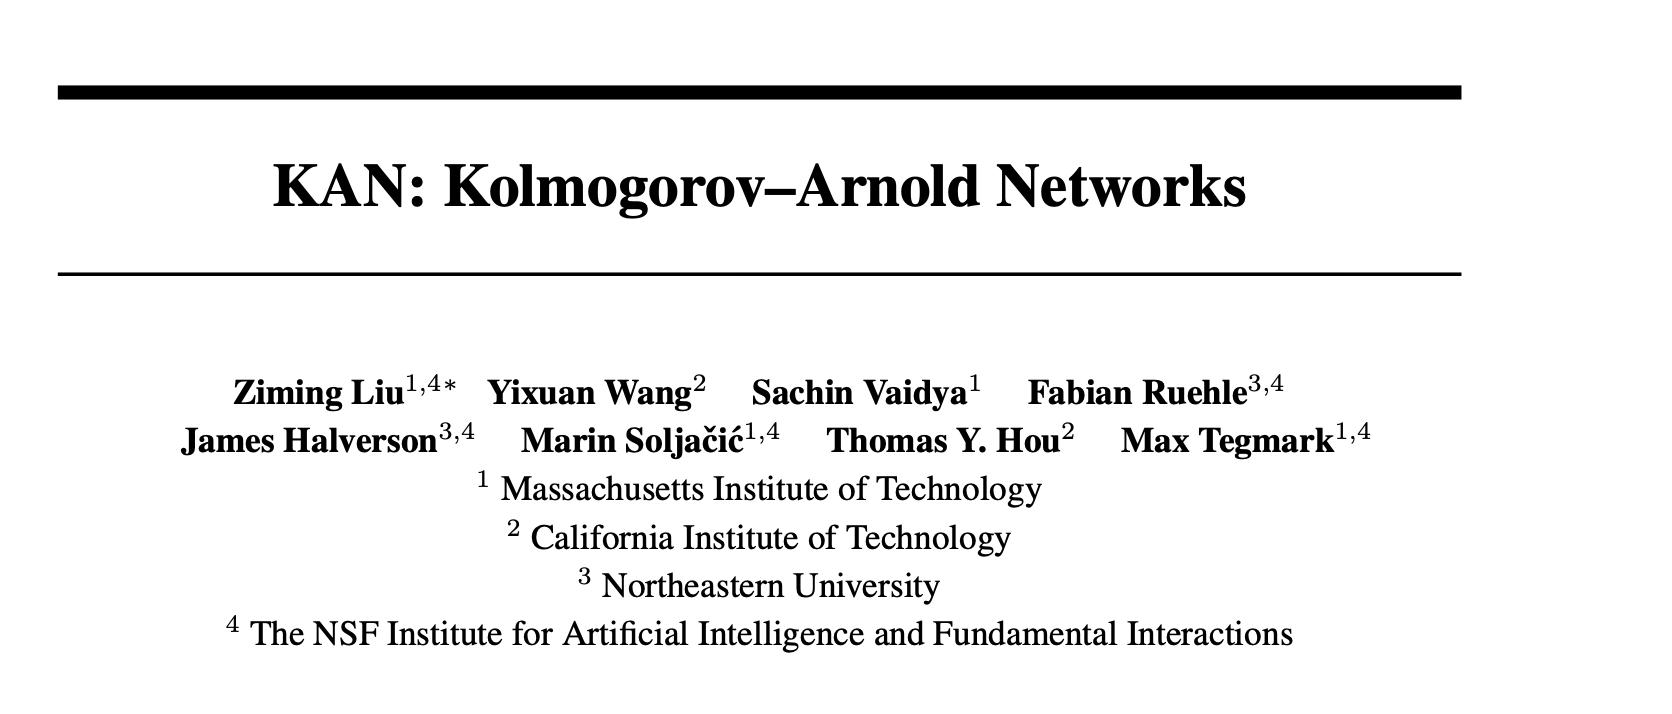
\includegraphics[width=3.9in]{assets/ClassicKAN.png}}
    \tb{3.9}{8.99}{2.55}{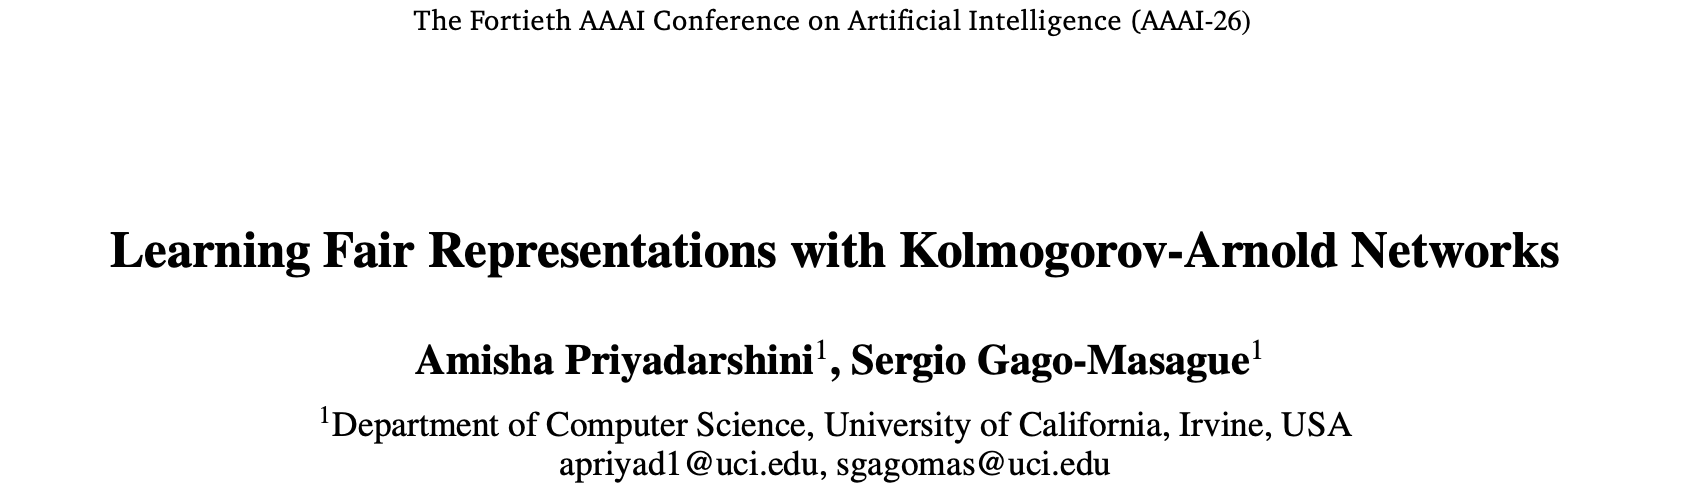
\includegraphics[width=3.9in]{assets/fairKAN.png}}
    \tb[align=center]{3.9}{0.45}{4.35}{\color{body}\fs{12}{14}\textbf{Kolmogorov-Arnold Networks}\par\smallskip
      Activation functions are placed on edges instead of nodes.}
    \tb[align=center]{3.9}{4.72}{4.35}{\color{body}\fs{12}{14}\textbf{$D^3$KAN}\par\smallskip
      A denoising and data-complexity-adaptive KAN for long-term forecasting.}
    \tb[align=center]{3.9}{8.99}{4.35}{\color{body}\fs{12}{14}\textbf{Learning Fair Representations with KANs}\par\smallskip
      KANs applied to learning fair representations.}
\end{frame}

% ===================================================== LAMBDA CONTROLLER (06)
\pageset{The $\lambda$ controller}{03}
\begin{frame}
  \ctitle{\normalsize We change the objective function from $\mathcal{L} + \lambda \mathcal{P}(\theta)$ to $\min_{\theta} \mathcal{L}(\theta)$ s.t. $DP(\theta) <= \epsilon$ 
  so we can ensure more flexibility during drift and avoid the need for a per dataset tunable hyperparameter $\lambda$}
\begin{center}
  \begin{theorem}
    \centering
    $\min_{\theta} \mathcal{L}(\theta)$ s.t. $DP(\theta) <= \epsilon$ is equivalent to $\min_{\theta}\max_{\mu >= 0}\mathcal{L}$
  \end{theorem}
\end{center}
\begin{proof}
  Let $DP = max_g|D_g|, D_g = \hat{r} - r_{g}$ where $r_{g}$ is group g's positive-prediction rate and 
  $\hat{r}$ is the mean of those rates (e.g. with two groups deviations are always mirror images meaning $D_{0} = -D_{1}$). Using the fact that 
  $|x| \leq \epsilon \equiv -x \leq \epsilon \land x \leq \epsilon$ then we can rewrite $|D_g| \leq \epsilon$ as $D_g \leq \epsilon$ and $D_g \geq -\epsilon$ : Same requirement 
  without absolute value and, additionally, we know which side is beeing violated.
  
  We can now rewrite the Loss function using the Lagrange multiplier $\mu$ as follows:
  $\mathcal{L}(\theta, \mu) = \mathcal{L}(\theta) + \sum_{g} (\mu_{g+}(D_g - \epsilon) + \mu_{g-}(-D_g - \epsilon))$
  with $\mu_k \geq 0, \forall \mu_k$.

  If we assume a fair classifier where $DP - \epsilon \leq 0$ then $\mu(DP - \epsilon) \to -\infty$ as $\mu$ increases, whereas 
  if we assume an unfair classifier where $DP - \epsilon > 0$ then $\mu(DP - \epsilon) \to +\infty$. 
  Therefore, the Lagrange multiplier $\mu$ will be maximized when the classifier is unfair and minimized when the classifier is fair. 
  This means that the optimization problem can be reformulated as a min-max problem, where we minimize the loss function with respect 
  to the model parameters $\theta$ while maximizing it with respect to the Lagrange multiplier $\mu$ (if we instead chose to minimize
  the $\mu$ player would just choose 0 everytime). This leads to the equivalent formulation:
  \begin{center}
    $\min_{\theta}\max_{\mu >= 0}\mathcal{L}(\theta, \mu)$.
  \end{center}
\end{proof}
This also means we can find the price, $\mu$, by dual ascent making $\lambda$ adaptative, dataset agnostic and not requiring hyperparameter tuning. 
This is a more flexible approach that allows the model to adapt to changing conditions and ensure fairness without the need for 
manual tuning of $\lambda$. The dual ascent finds the optimal value of $\mu$ in the following way:
\begin{center}
  $\frac{\partial\mathcal{L}}{\partial\mu_{g_{\pm}}}$ $=$ $\pm(D_g-\epsilon)$.
\end{center}

Updating $\mu$ as: $\mu_{g_{\pm}}$ = clip$(\mu_{g_{\pm}} + \eta(\pm D_g -\epsilon), 0, \lambda_{\max})$ where $\eta$ is the learning rate 
and $\lambda_{\max}$ is the maximum value of $\lambda$ (which we can set to infinity). This way we keep non-negative prices and
bound the duality requirement + accuracy trade-off. 
\end{frame}

\pageset{The $\lambda$ controller}{04}
\begin{frame}
  \frametitle{The $\lambda$ controller}
  \ctitle{\normalsize How can we estimate $D_g$?}
  We see one person at a time ($a_t$, $\hat{y}_t$), which is not a meaningful rate for every group - we need to be right on average.
  The Horvitz-Thompson estimator states:
  \begin{center}
    Let $Y_i, i = 1, \ldots, n$ be an independent sample from n of N >= n distinct stratum with mean $\mu$.
    Supose $\pi_i$ is the inclusion probability (i.e. sample belongs to the i-th stratum) then:
    $\hat{Y}_{HT} = \sum_{i=1}^{n} \frac{Y_i}{\pi_i}$ and mean estimate $\hat{\mu}_{HT} = \frac{1}{N}\sum_{i=1}^{n} \frac{Y_i}{\pi_i}$ is unbiased for $\mu$.
  \end{center}
  In our case, we want to estimate $r_g$ (equal it on average) and we can use the Horvitz-Thompson estimator to do so. We can estimate $r_g$ as follows:
  \begin{center}
    $u_{t,g}$ = $\frac{\hat{y}_t = 1}{\pi_g}$ with probability $\pi_g \times r_g$ otherwise 0. 
  \end{center}
  On average: 
  \begin{center}
    $\pi_g \times r_g \times u_{t,g}$ = $r_g$
  \end{center}
  \begin{theorem}
    \centering
      $\mathbb{E}[v]$ = $D_g$: The estimator is right on average.
  \end{theorem}

  \begin{proof}
    Let the estimator $v_{t, g}$ be defined as $\frac{1}{G}\sum_h(u_{t,h} - u_{t,g})$.
    Because $\mathbb{E}[u_{t,g}]$ = $\frac{1}{\pi_g}(\pi_g \times r_g) + 0(1 - \pi_g \times r_g)$ = $r_g$, we have:

    \begin{center}
      $\mathbb{E}[v_{t,g}]$ = $\frac{1}{G}\sum_h(\mathbb{E}[u_{t,h}] - \mathbb{E}[u_{t,g}])$ = $\frac{1}{G}\sum_h(r_h - r_g)$ = $\hat{r} - r_g$ = $D_g$.
    \end{center}
    And thus we prove that the estimator is right on average.
  \end{proof}
  \slidefoot{Limitations: Samples are independent given the model but not identically distributed (in online learning model's distribution changes over time)}
\end{frame}

\end{document}
